\documentclass{article}
\usepackage{graphicx,fullpage,float}
\begin{document}

\pagebreak
\begin{center}
	\textbf{Journalist's Strategy}
\end{center}
\begin{figure}[h]
	\begin{center}
		\begin{tabular}{cc}
			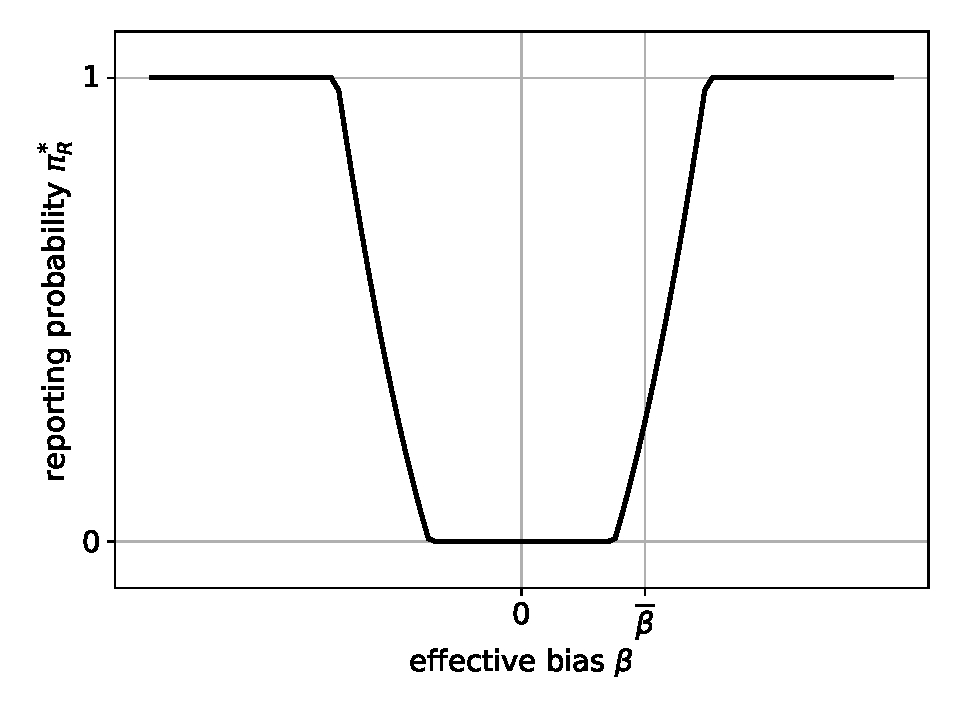
\includegraphics[scale=.5]{effective_bias_reporting_probability} & 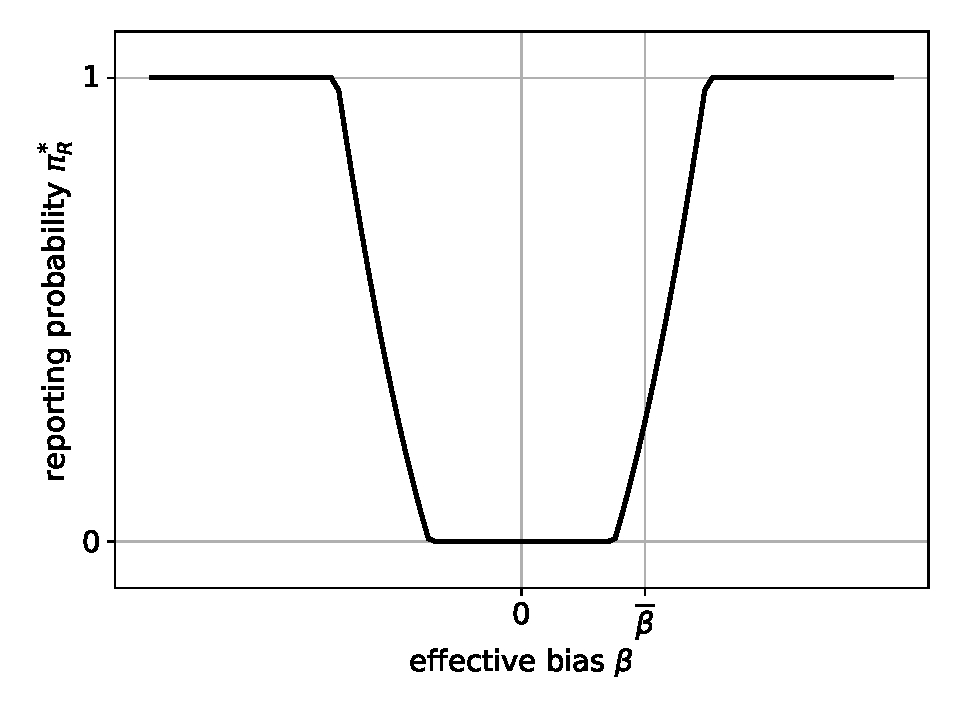
\includegraphics[scale=.5]{effective_bias_reporting_probability} \\
		\end{tabular}
	\end{center}
\end{figure}

\pagebreak
\begin{center}
	\textbf{Equilibrium Actions}
\end{center}
\begin{figure}[h]
	\begin{center}
		\begin{tabular}{cc}
			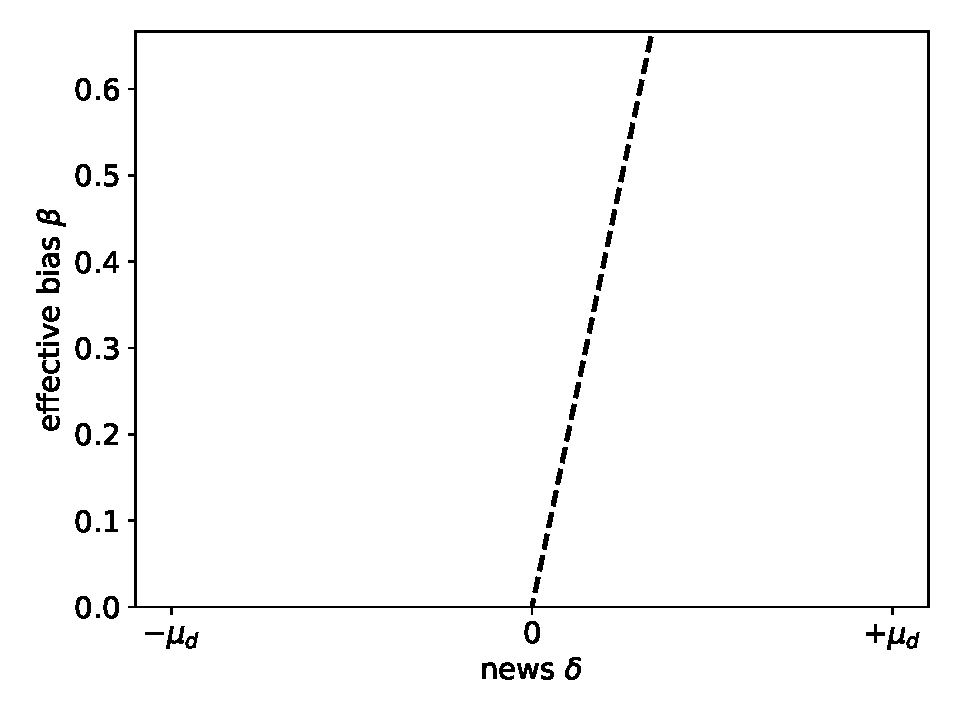
\includegraphics[scale=.5]{news_effective_bias} & 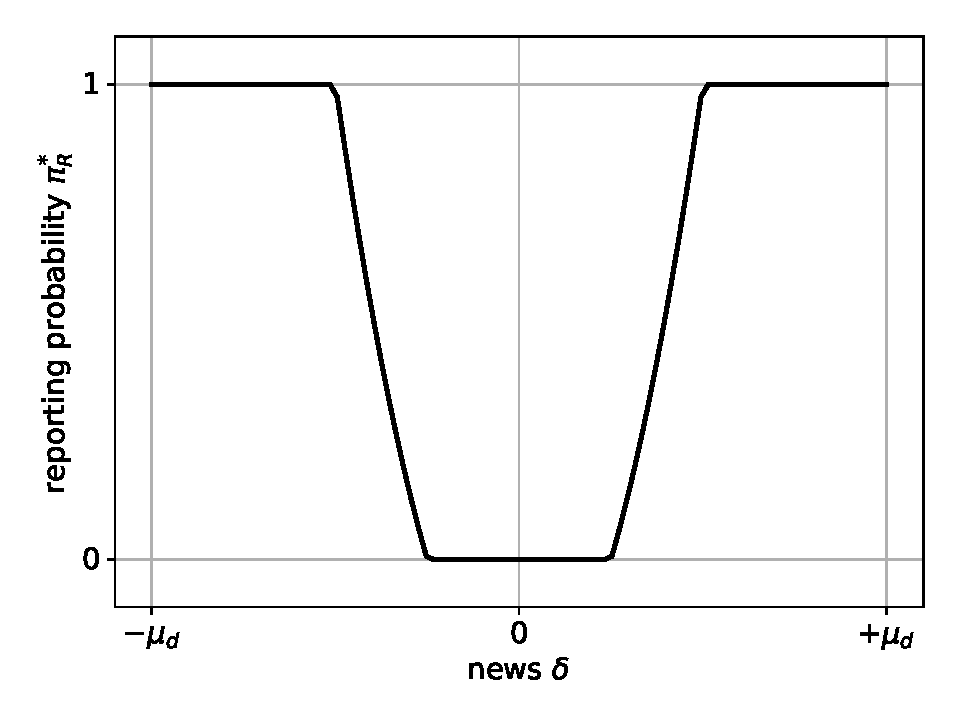
\includegraphics[scale=.5]{news_reporting_probability} \\
		\end{tabular}
	\end{center}
\end{figure}

\pagebreak
\begin{center}
	\textbf{Reports}
\end{center}
\begin{figure}[h]
	\begin{center}
		\begin{tabular}{cc}
			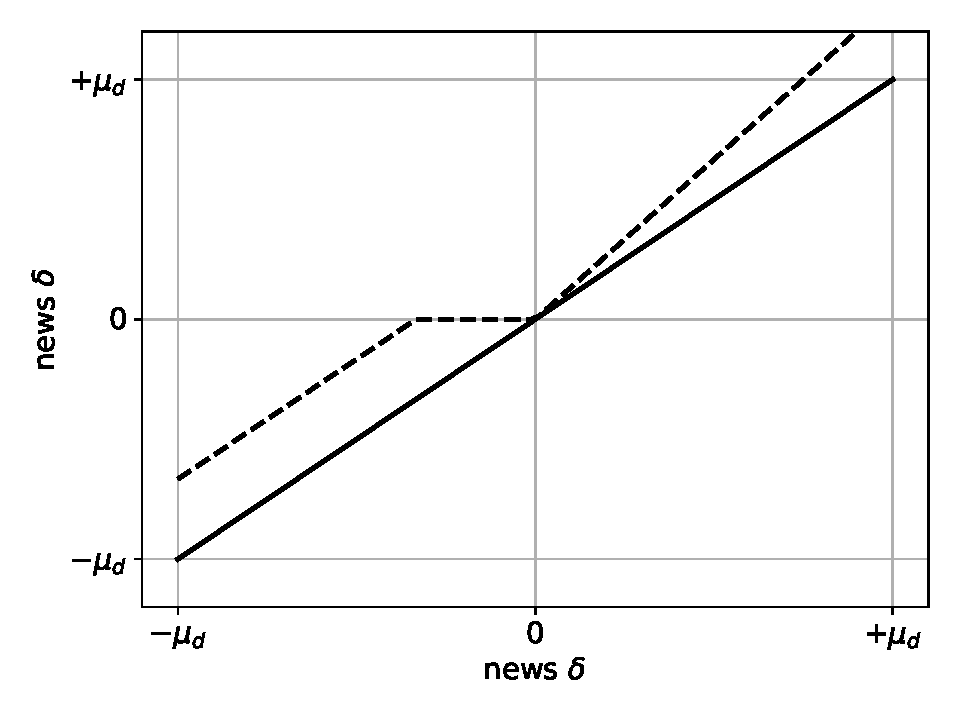
\includegraphics[scale=.5]{news_news_managers_report} & 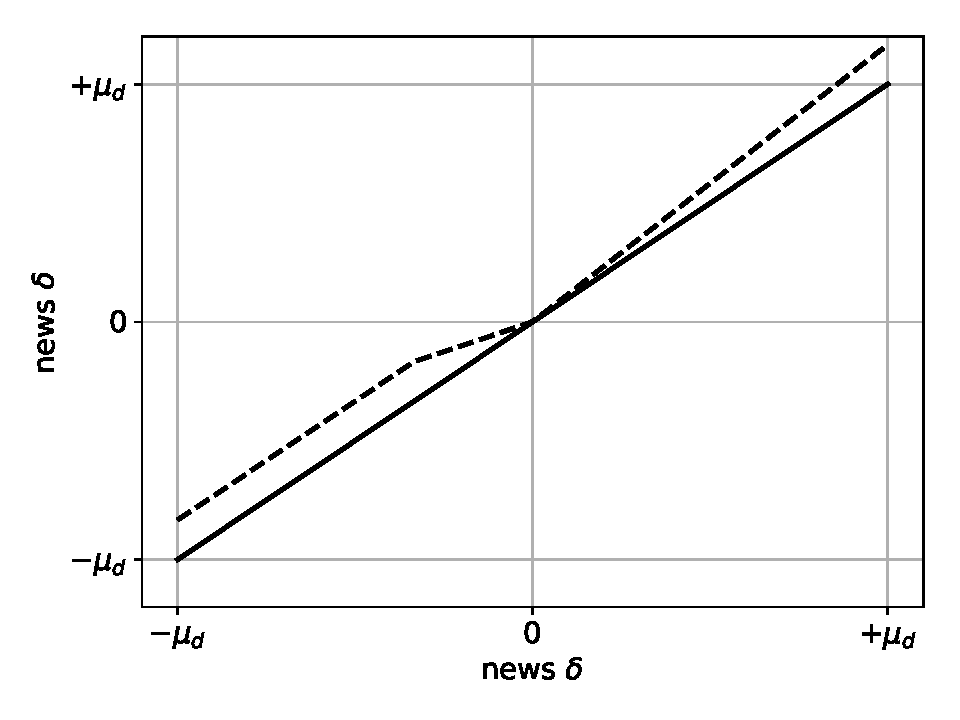
\includegraphics[scale=.5]{news_news_journalist_report} 
		\end{tabular}
	\end{center}
\end{figure}

\pagebreak
\begin{center}
	\textbf{Market Outcomes}
\end{center}
\begin{figure}[h]
	\begin{center}
		\begin{tabular}{cc}
			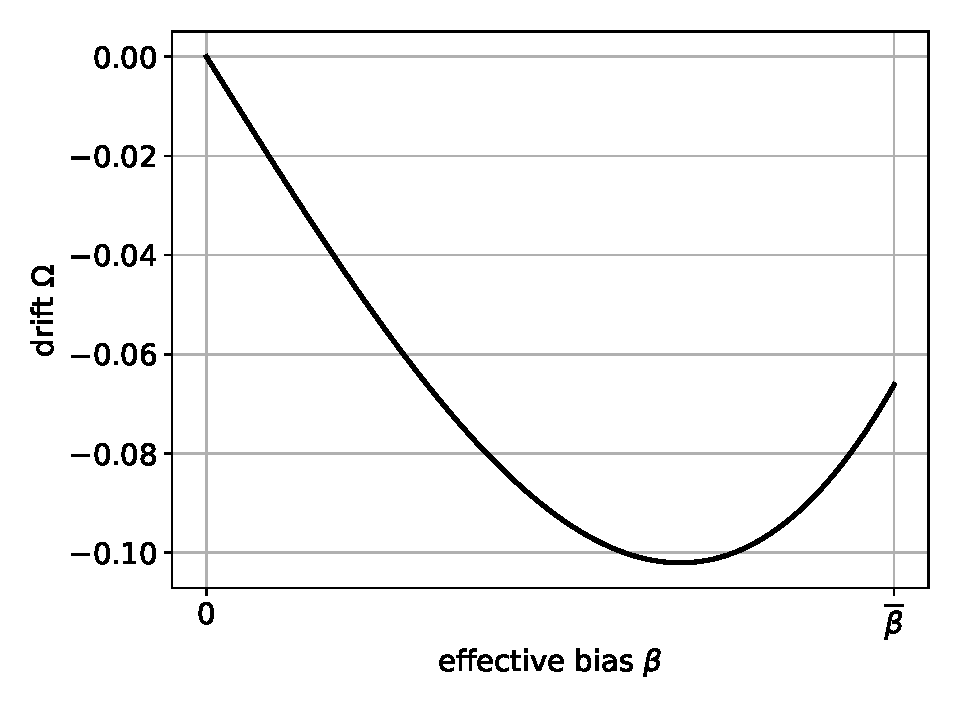
\includegraphics[scale=.5]{effective_bias_drift} & 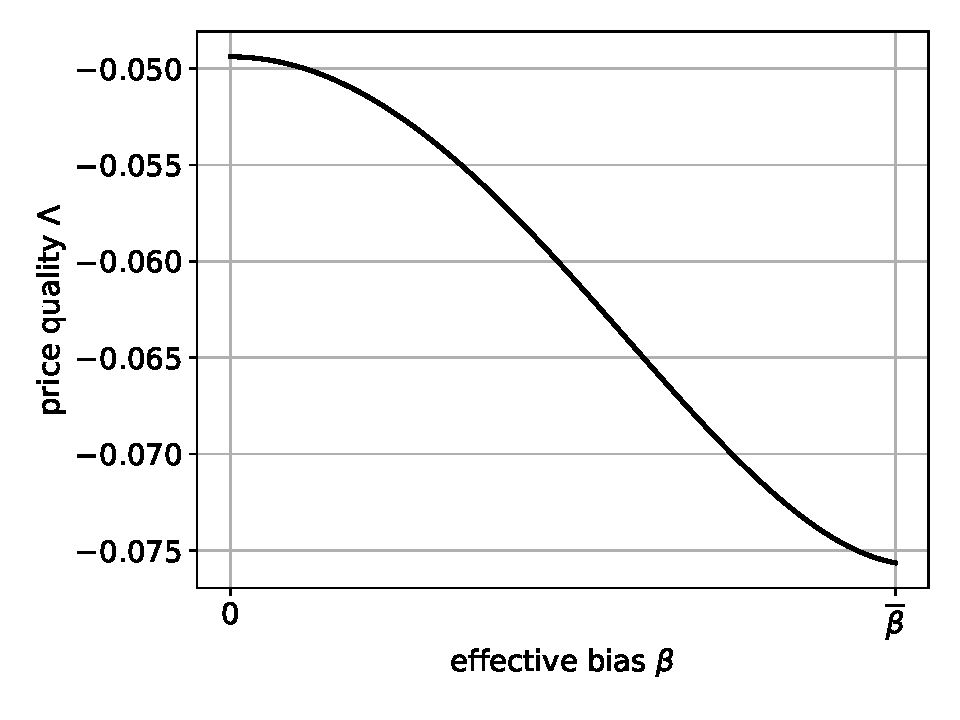
\includegraphics[scale=.5]{effective_bias_price_quality} \\
			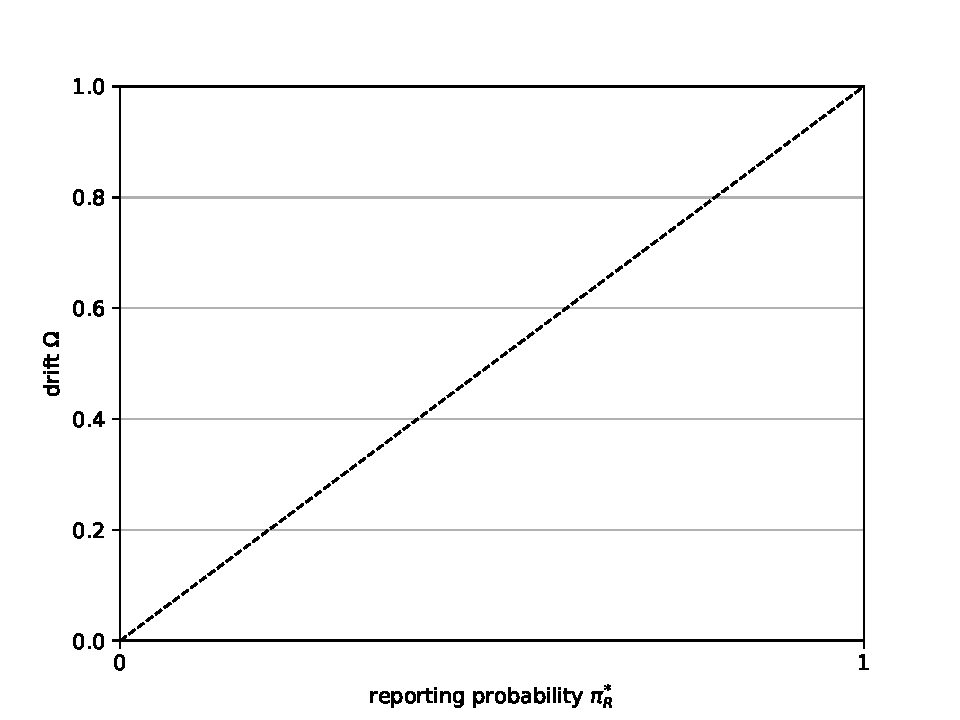
\includegraphics[scale=.5]{reporting_probability_drift} & 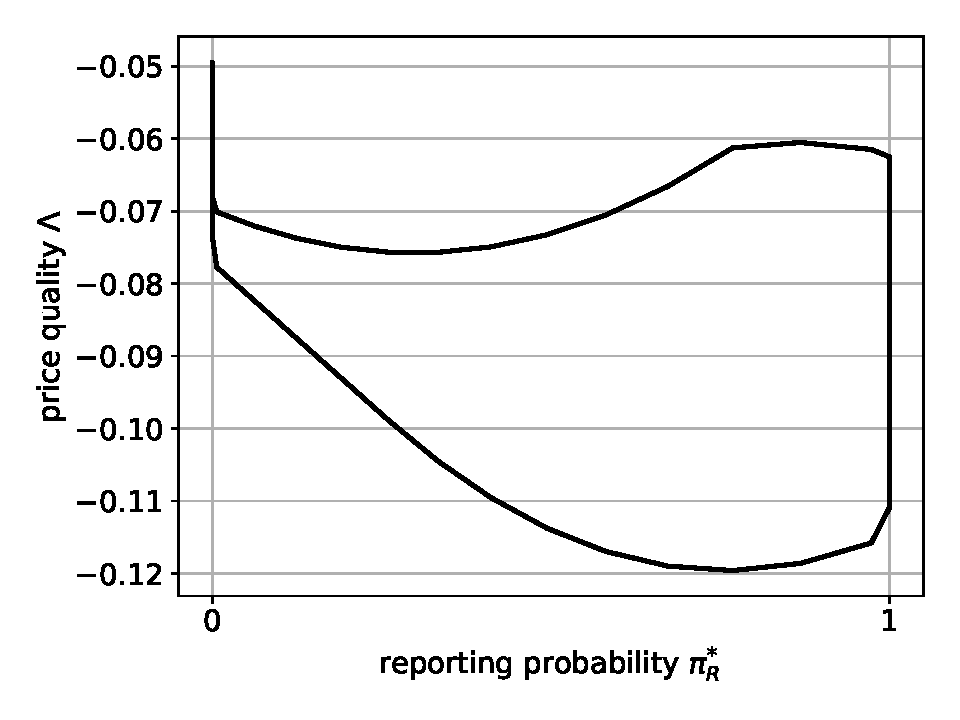
\includegraphics[scale=.5]{reporting_probability_price_quality} 
		\end{tabular}
	\end{center}
\end{figure}

\pagebreak
\begin{center}
	\textbf{Loss Aversion}
\end{center}
\begin{figure}[h]
	\begin{center}
		\begin{tabular}{c}
			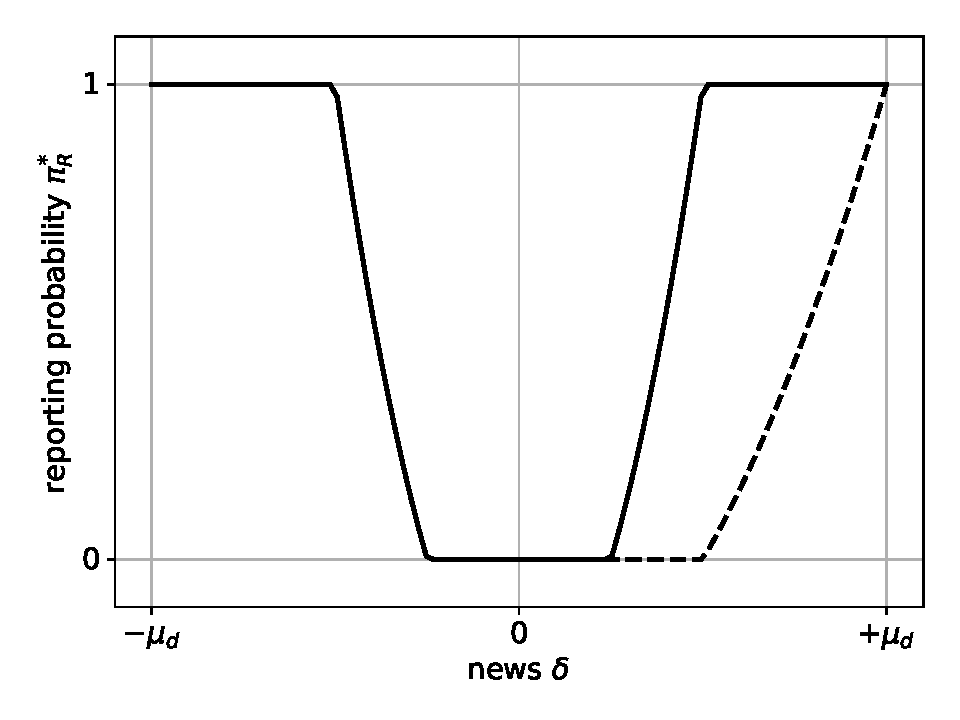
\includegraphics[scale=.5]{news_reporting_probability_reporting_probability} 
		\end{tabular}
	\end{center}
\end{figure}

\end{document}
